% Options for packages loaded elsewhere
\PassOptionsToPackage{unicode}{hyperref}
\PassOptionsToPackage{hyphens}{url}
\PassOptionsToPackage{dvipsnames,svgnames,x11names}{xcolor}
%
\documentclass[
  number]{elsarticle}

\usepackage{amsmath,amssymb}
\usepackage{iftex}
\ifPDFTeX
  \usepackage[T1]{fontenc}
  \usepackage[utf8]{inputenc}
  \usepackage{textcomp} % provide euro and other symbols
\else % if luatex or xetex
  \usepackage{unicode-math}
  \defaultfontfeatures{Scale=MatchLowercase}
  \defaultfontfeatures[\rmfamily]{Ligatures=TeX,Scale=1}
\fi
\usepackage{lmodern}
\ifPDFTeX\else  
    % xetex/luatex font selection
\fi
% Use upquote if available, for straight quotes in verbatim environments
\IfFileExists{upquote.sty}{\usepackage{upquote}}{}
\IfFileExists{microtype.sty}{% use microtype if available
  \usepackage[]{microtype}
  \UseMicrotypeSet[protrusion]{basicmath} % disable protrusion for tt fonts
}{}
\makeatletter
\@ifundefined{KOMAClassName}{% if non-KOMA class
  \IfFileExists{parskip.sty}{%
    \usepackage{parskip}
  }{% else
    \setlength{\parindent}{0pt}
    \setlength{\parskip}{6pt plus 2pt minus 1pt}}
}{% if KOMA class
  \KOMAoptions{parskip=half}}
\makeatother
\usepackage{xcolor}
\setlength{\emergencystretch}{3em} % prevent overfull lines
\setcounter{secnumdepth}{5}
% Make \paragraph and \subparagraph free-standing
\makeatletter
\ifx\paragraph\undefined\else
  \let\oldparagraph\paragraph
  \renewcommand{\paragraph}{
    \@ifstar
      \xxxParagraphStar
      \xxxParagraphNoStar
  }
  \newcommand{\xxxParagraphStar}[1]{\oldparagraph*{#1}\mbox{}}
  \newcommand{\xxxParagraphNoStar}[1]{\oldparagraph{#1}\mbox{}}
\fi
\ifx\subparagraph\undefined\else
  \let\oldsubparagraph\subparagraph
  \renewcommand{\subparagraph}{
    \@ifstar
      \xxxSubParagraphStar
      \xxxSubParagraphNoStar
  }
  \newcommand{\xxxSubParagraphStar}[1]{\oldsubparagraph*{#1}\mbox{}}
  \newcommand{\xxxSubParagraphNoStar}[1]{\oldsubparagraph{#1}\mbox{}}
\fi
\makeatother


\providecommand{\tightlist}{%
  \setlength{\itemsep}{0pt}\setlength{\parskip}{0pt}}\usepackage{longtable,booktabs,array}
\usepackage{calc} % for calculating minipage widths
% Correct order of tables after \paragraph or \subparagraph
\usepackage{etoolbox}
\makeatletter
\patchcmd\longtable{\par}{\if@noskipsec\mbox{}\fi\par}{}{}
\makeatother
% Allow footnotes in longtable head/foot
\IfFileExists{footnotehyper.sty}{\usepackage{footnotehyper}}{\usepackage{footnote}}
\makesavenoteenv{longtable}
\usepackage{graphicx}
\makeatletter
\newsavebox\pandoc@box
\newcommand*\pandocbounded[1]{% scales image to fit in text height/width
  \sbox\pandoc@box{#1}%
  \Gscale@div\@tempa{\textheight}{\dimexpr\ht\pandoc@box+\dp\pandoc@box\relax}%
  \Gscale@div\@tempb{\linewidth}{\wd\pandoc@box}%
  \ifdim\@tempb\p@<\@tempa\p@\let\@tempa\@tempb\fi% select the smaller of both
  \ifdim\@tempa\p@<\p@\scalebox{\@tempa}{\usebox\pandoc@box}%
  \else\usebox{\pandoc@box}%
  \fi%
}
% Set default figure placement to htbp
\def\fps@figure{htbp}
\makeatother

\makeatletter
\@ifpackageloaded{float}{}{\usepackage{float}}
\floatstyle{plain}
\@ifundefined{c@chapter}{\newfloat{suppfig}{h}{losuppfig}}{\newfloat{suppfig}{h}{losuppfig}[chapter]}
\floatname{suppfig}{Figure S}
\newcommand*\quartosuppfigref[1]{Figure \hyperref[#1]{S\ref{#1}}}
\@ifpackageloaded{caption}{}{\usepackage{caption}}
\DeclareCaptionLabelFormat{quartosuppfigreflabelformat}{#1#2}
\captionsetup[suppfig]{labelformat=quartosuppfigreflabelformat}
\newcommand*\listofsuppfigs{\listof{suppfig}{List of Supplementary Figures}}
\makeatother
\makeatletter
\@ifpackageloaded{float}{}{\usepackage{float}}
\floatstyle{plain}
\@ifundefined{c@chapter}{\newfloat{supptab}{h}{losupptab}}{\newfloat{supptab}{h}{losupptab}[chapter]}
\floatname{supptab}{Table S}
\newcommand*\quartosupptabref[1]{Table \hyperref[#1]{S\ref{#1}}}
\@ifpackageloaded{caption}{}{\usepackage{caption}}
\DeclareCaptionLabelFormat{quartosupptabreflabelformat}{#1#2}
\captionsetup[supptab]{labelformat=quartosupptabreflabelformat}
\newcommand*\listofsupptabs{\listof{supptab}{List of Supplementary Tables}}
\makeatother
\makeatletter
\@ifpackageloaded{caption}{}{\usepackage{caption}}
\AtBeginDocument{%
\ifdefined\contentsname
  \renewcommand*\contentsname{Table of contents}
\else
  \newcommand\contentsname{Table of contents}
\fi
\ifdefined\listfigurename
  \renewcommand*\listfigurename{List of Figures}
\else
  \newcommand\listfigurename{List of Figures}
\fi
\ifdefined\listtablename
  \renewcommand*\listtablename{List of Tables}
\else
  \newcommand\listtablename{List of Tables}
\fi
\ifdefined\figurename
  \renewcommand*\figurename{Figure}
\else
  \newcommand\figurename{Figure}
\fi
\ifdefined\tablename
  \renewcommand*\tablename{Table}
\else
  \newcommand\tablename{Table}
\fi
}
\@ifpackageloaded{float}{}{\usepackage{float}}
\floatstyle{ruled}
\@ifundefined{c@chapter}{\newfloat{codelisting}{h}{lop}}{\newfloat{codelisting}{h}{lop}[chapter]}
\floatname{codelisting}{Listing}
\newcommand*\listoflistings{\listof{codelisting}{List of Listings}}
\makeatother
\makeatletter
\makeatother
\makeatletter
\@ifpackageloaded{caption}{}{\usepackage{caption}}
\@ifpackageloaded{subcaption}{}{\usepackage{subcaption}}
\makeatother

\usepackage[]{natbib}
\bibliographystyle{elsarticle-num}
\usepackage{bookmark}

\IfFileExists{xurl.sty}{\usepackage{xurl}}{} % add URL line breaks if available
\urlstyle{same} % disable monospaced font for URLs
\hypersetup{
  pdftitle={Preliminary Investigation of Spatial Variability of Sediment Fingerprinting Properties in Relation to Terrain Attributes at the Field-Scale},
  pdfauthor={Maria Luna Miño; Alexander J Koiter; Taras E Lychuk; Arnie Waddel; Alan Moulin},
  pdfkeywords={Soil geochemistry, Soil colour, Spatial analysis, Terrain
attributes},
  colorlinks=true,
  linkcolor={blue},
  filecolor={Maroon},
  citecolor={Blue},
  urlcolor={Blue},
  pdfcreator={LaTeX via pandoc}}


\setlength{\parindent}{6pt}
\begin{document}

\begin{frontmatter}
\title{Preliminary Investigation of Spatial Variability of Sediment
Fingerprinting Properties in Relation to Terrain Attributes at the
Field-Scale}
\author[1]{Maria Luna Miño%
%
}
 \ead{LUNAMIMA56@brandonu.ca} 
\author[2]{Alexander J Koiter%
\corref{cor1}%
}
 \ead{koitera@brandonu.ca} 
\author[3]{Taras E Lychuk%
%
}
 \ead{taras.lychuk@AGR.GC.CA} 
\author[3]{Arnie Waddel%
%
}
 \ead{arnie.waddell@AGR.GC.CA} 
\author[3]{Alan Moulin%
%
}
 \ead{apmaafc7788@gmail.com} 

\affiliation[1]{organization={Brandon University, Masters in
Environmental and Life Sciences},addressline={270 18th
St},city={Brandon},postcode={R7A 6A9},postcodesep={}}
\affiliation[2]{organization={Brandon University, Department of
Geography and Environment},addressline={270 18th
St},city={Brandon},postcode={R7A 6A9},postcodesep={}}
\affiliation[3]{organization={Agriculture and Agri-Food Canada, Brandon
Research and Development Centre},addressline={2701 Grand Valley
Road},city={Brandon},postcode={R7A 5Y3},postcodesep={}}

\cortext[cor1]{Corresponding author}





        
\begin{abstract}
Quantifying field-scale (∼40 ha) spatial variability in soil geochemical
and colour (spectral reflectance) properties is important for sediment
source fingerprinting. The main objectives of this study were to: 1)
quantify the spatial variability and spatial dependence for a set of 15
properties (10 geochemical elements: Ca, Co, Cs, Fe, Li, La, Nb, Ni, Rb,
Sr; and 5 colour coefficients: \emph{a*, b*, c*, h*}, and \emph{x})
measured from the \textless63 μm fraction at an agricultural and
forested site; and 2) assess how seven terrain attributes (elevation,
SAGA wetness index, relative slope position, catchment area, vertical
distance to channel network, plan curvature, profile curvature) relate
to these properties through correlation and Random Forest (RF)
regression. Across both sites, colour properties exhibited approximately
normal distributions with low coefficients of variation (CV), whereas
geochemical properties were more variable and skewed. Semivariograms
indicated strong spatial dependence for most properties at the
agricultural site (median range ≈ 210 m) and moderate dependence at the
forested site (ranges 176--298 m). RF models performed better at the
agricultural site; elevation, wetness and slope position were the
top-ranked predictors for most properties. These results support
DEM-based sampling strategies. In practice, sample spacing on the order
of the semivariogram range (∼200--230 m) can suffice for mapping in
simple agricultural settings, whereas stratified designs (e.g.,
near-stream vs.~hillslope) may be preferable in more complex forested
terrains.
\end{abstract}





\begin{keyword}
    Soil geochemistry \sep Soil colour \sep Spatial analysis \sep 
    Terrain attributes
\end{keyword}
\end{frontmatter}
    

\subsection{Introduction}\label{introduction}

Spatial variation in soil properties arises from soil-forming factors
(parent material, relief, biota, climate, time) and is further modified
by land use and management practices. Characterizing the patterns and
drivers of this variation is an important component of many
agri-environmental studies. For example, to meet the desired level of
precision for agronomic and environmental nutrient management plans the
spatial variability in soil nutrients will influence the soil sampling
design in terms of number and locations of soil samples (Kariuki et al.,
2009; Starr et al., 1995). Similarly, accounting for spatial variability
extends to sediment source fingerprinting, as unaccounted spatial
heterogeneity within sources of sediment can compromise the source
apportionment results (Du and Walling, 2017).

Sediment source fingerprinting is a watershed-scale technique that is
used to quantify the relative proportions of sediment derived from
unique sources. This technique uses naturally occurring biogeochemical
properties as fingerprints (i.e., tracers) to link potential sources of
sediment to downstream sediment. Investigating the spatial variability
at a watershed-scale can be advantageous to identify, classify, and
distinguish between potential sources of sediment (Pulley et al., 2017).
However, investigating spatial variability at smaller scales is less
common (e.g., Du and Walling, 2017; Pulley et al., 2018; Collins et al.,
2019; Luna Miño et al., 2024) and remains a research priority (Collins
et al., 2020). Within the sediment source fingerprinting approach
field-scale (\textless1 km²) variability is important for (i) designing
efficient, representative source sampling, (ii) integrating spatial
variability with erosion/delivery gradients for mixing models, and (iii)
selecting fingerprints supported by process-based reasoning. Previous
work has highlighted spatial variability issues and the need for more
robust, process-informed fingerprint selection and sampling strategies.

Characterization of fingerprint properties requires representative
sampling, particularly because variability in some properties is not
random but follows systematic spatial patterns across the landscape. For
example, the pattern of fallout radionuclides will reflect the long-term
patterns of soil erosion and deposition (Wilkinson et al., 2015).
Designing and implementing source sampling campaigns must consider this,
as the sampling design used has been shown to influence the
characterization of a wide range of commonly used fingerprints (Luna
Miño et al., 2024). The lack of standardization in sediment source
sampling designs makes it difficult to compare results across studies
and creates uncertainties in the interpretation of results (Luna Miño et
al., 2024)

Characterization of sources is further complicated by variations in
erosion and sediment delivery rates across the landscape. Many mixing
models use well defined inputs (sources) and outputs (sediment)
characterized by mean and standard deviation, but do not consider the
spatial distribution of fingerprint properties. This is a limitation of
the methodology as samples collected closer to and more hydrologically
connected with the stream network may better represent the source, even
if they deviate from the mean value. Strategic/judgment sampling
targeting the likely to eroded areas may improve representativeness, but
it prevents an overview of the broader spatial patterns, limiting the
interpretation of landscape processes across the entire source area.
There has been progress using information on erosion rates to calculate
an erosion rate-weighted mean (Wilkinson et al., 2015; Du and Walling,
2017) and using spatially interpolated maps of fingerprint values to
provide a finer resolution of the fingerprint variability within each
source (Haddadchi et al., 2019). Characterizing the geomorphic,
hydrologic, and biochemical processes underlying spatial variability
supports the selection of reliable fingerprints and informs sampling
design for source characterization. While many studies use a
statistical-based approach (Collins et al., 1997) to select suitable
fingerprints there are concerns that this approach may result in the
inclusion of false positives (i.e., type I error) in which a fingerprint
is incorrectly identified as having discriminatory power between sources
when it does not, or non-conservative fingerprints (Koiter et al.,
2013a). Consequently, there has been a call for the inclusion of a
process-based (e.g., weathering, erosion) or geologic-based explanation
of the fingerprints selected to address these concerns (Collins et al.,
2020). This remains challenging due to limited data on soil properties,
particularly with geochemical properties, as routine lab analysis often
measures more than 50 elements. The spatial patterns of some soil
properties are well studied because of their agronomic importance or
ability to infer other important soil properties and processes and
include fallout radionuclides (e.g., \textsuperscript{137}Cs, 7Be;
Ritchie et al.~1970), plant nutrients (e.g., N, P; Vasu et al.~2017),
soil colour (e.g., hue, value; Viscarra Rossel et al.~2006), major
non-acid forming cations (e.g., Ca, Na; Sun et al.~2021a). In contrast,
the processes that control the distribution of rare earth elements and
trace metals, are less well studied or tend to be site-specific, making
it difficult to draw generalizations.

Terrain attributes such as elevation, slope curvature, slope position,
and soil wetness indices have been shown to be useful information in the
characterization and modelling of a range of soil properties including
soil moisture (Beaudette et al., 2013), texture (Kokulan et al., 2018),
colour (Brown et al., 2004), organic matter (Zhang et al., 2012),
conductivity (Umali et al., 2012), and geochemistry (Lima et al., 2023).
Similar techniques may provide additional insight into the pedologic and
geomorphic processes that drive the observed patterns of fingerprint
properties within a given source. Digital elevation models (DEMs) are
more widely available through public databases and can be generated
using drone imagery, whereas soil property data are more limited in
availability and spatial coverage. As a result, terrain attributes
derived from DEMs offer a practical and more readily available basis for
guiding efficient and spatially informed soil sampling designs. This
study builds on the previous work of Luna Miño (2024) where the impact
of three different sampling designs on the characterization of source
materials, within the framework of the sediment fingerprinting approach,
was assessed. This study expands that study by using the data from grid
sampling approach to assess the spatial autocorrelation, and identify
important terrain attributes driving the observed patterns. The
objectives of this study were to: (1) quantify the spatial variability
and spatial dependence of 15 fingerprint-relevant soil properties across
an agricultural and forested field site; and (2) test the relation
between these soil properties and seven terrain attributes (derived from
DEMs), using correlation and Random Forest regression to identify
terrain controls and their relative importance. Together, these
objectives address how terrain attributes may be used to understand
spatial distributions of soil properties and help guide sampling design.

\subsection{Methods}\label{methods}

\subsubsection{Site description}\label{site-description}

Two sites within \textasciitilde4 km of each other in the Wilson Creek
Watershed (WCW), near McCreary, Manitoba, Canada were sampled
(Figure~\ref{fig-location_map}). The mixedwood forest site (50°43'35''N,
99°33'36''W; 369.2 masl) in Riding Mountain National Park consists of
white spruce (Picea glauca), black spruce (Picea mariana), balsam fir
(Abies balsamea), larch (Larix laricina), and trembling aspen (Populus
tremuloides), with soils likely part of the Grey Wooded soil association
(Luvisol) developed on boulder till of mostly shale with some limestone
and granitic rocks (Ehrlich et al., 1958). This site has a local relief
of 17.9 m and moderately complex terrain, dissected by Wilson Creek, a
meandering stream with a gradient of approximately 0.006 m m-1,
featuring a small floodplain 5 to 25 m wide and adjacent upland areas
(Figure~\ref{fig-location_map}). The agricultural site (50°45'15''N,
99°30'49''W; 309.9 masl) includes grain and forage rotations and is
mapped to the Edwards Soil Series (Cumulic Regosol) with silty clay loam
to silty clay soils developed on alluvial deposits (Ehrlich et al.,
1958). The site has relatively simple terrain with a local relief of 2.8
m and drains toward the northeast corner of the field, where Wilson
Creek runs along the northern edge as a straight, engineered channel
(Figure~\ref{fig-location_map}). The region has a Dfb climate (Beck et
al., 2018), with a mean annual temperature of 3.0°C, annual
precipitation of 539 mm (\textasciitilde27\% as snow) (Environment and
Canada, 2024), and snowmelt-dominated runoff, with about 80\% occurring
in May and June (MacKay, 1970).

\begin{figure}[H]

\centering{

\pandocbounded{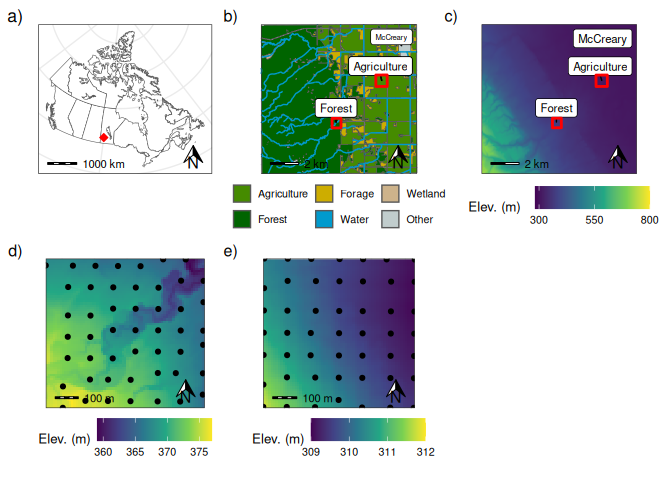
\includegraphics[keepaspectratio]{index_files/figure-latex/notebooks-location_map-fig-location_map-output-2.png}}

}

\caption{\label{fig-location_map}a) Map showing the location of the
study sites within Canada. Location of the two study sites and nearby
town of McCreary, and regional b) land use, and c) topography. Local
topography and soil sampling locations at the d) forested site and e)
agricultural site}

\end{figure}%

\textsubscript{Source:
\href{https://alex-koiter.github.io/terrain-attributes/notebooks/location_map.qmd.html\#cell-fig-location_map}{Research
Site Locations}}

\subsubsection{Soil sampling and
analysis}\label{soil-sampling-and-analysis}

At each site, 49 surface samples were collected on a 7×7 grid (100 m
spacing) (Figure~\ref{fig-location_map}). Forested samples were
collected 0--5 cm below the LFH to characterize the mineral A horizon,
minimizing organic layer heterogeneity; agricultural samples were 0--15
cm to reflect mixing by tillage and operations and to capture the
actively managed surface layer. Samples were dried, homogenized, and
sieved to \textless63 μm to minimize grain-size and organic matter
effects across sites and to align with established fingerprinting
protocols (Laceby et al., 2017). Samples were analyzed for a broad suite
of geochemical elements using aqua- regia digestion with ICP-MS (ALS
Mineral Division, North Vancouver, BC, Canada). Spectral measurements
were made with a spectroradiometer (ASD FieldSpecPro Malvern Panalytical
Inc Westborough MA 01581, United States). Spectral reflectance
measurements were taken in 1 nm increments over the 0.4-2.5 μm
wavelength range. Both samples and the Spectralon standard (white
reference) were illuminated with a white light source using a
halogen-based lamp (12 VDC, 20 Watt). Dark-current correction and white
reference were completed between samples. Fifteen colour coefficients
(\quartosupptabref{supptab-abbrev}) were computed from each sample,
where each sample represents the average of 10 spectra, following
published methods. (Koiter, 2021; Boudreault et al.~(2018). Based on the
results of Luna Miño (2024), a composite fingerprint consisting of 10
geochemical elements (Ca, Co, Cs, Fe, Li, La, Nb, Ni, Rb, and Sr) and
five colour coefficients (\emph{a*, b*, c*, h*,} and \emph{x}) were
identified as providing a strong discrimination between the agricultural
and forested surface soils. These fifteen soil properties are the focus
of the detailed spatial analysis detailed in this study.

\subsubsection{Geospatial and terrain
analysis}\label{geospatial-and-terrain-analysis}

All geostatistics were performed with ArcGIS Pro (v 3.3.0 Esri, 2024).
Semivariograms were used to quantify spatial correlation for each of the
15 soil properties. The optimization tool, based on minimizing the mean
square error, was used to parameterize the semivariogram model. In all
cases the Stable model type was used as it offers greater flexibility in
fitting the spatial correlation structure. The semivariograms were
visually inspected to ensure the automated fits were reasonable. Kriging
was used to interpolate and generate maps of each soil property. The
exploratory interpolation tool (Geostatistical Analyst extension) was
used to select the kriging type with the highest ranked prediction
accuracy. Cross-validation was used assess the performance of the
spatial interpolation and the measured and predicted values were plotted
and the r\textsuperscript{2} was reported.

The forested digital elevation model (DEM) was derived from Natural
Resources Canada's High-Resolution DEM Mosaic (HRDEM) (Natural Resources
Canada, 2024), while the agricultural DEM was generated using UAV
photogrammetry processed in Agisoft Metashape (v1.8.2 Agisoft, 2021)
with ground control points. Both DEMs were interpolated to 1 m
resolution grids using ordinary kriging. Terrain attributes including
elevation, plan and profile curvature, SAGA wetness index, catchment
area, relative slope position, and vertical distance to channel network
were computed in SAGA GIS (SAGA v2.1.4 Conrad et al., 2015)
(\quartosupptabref{supptab-terrain}). The native resolution between the
HRDEM and UAV-derived DEM differ, which may affect curvature metrics.
All rasters were resampled to 10 m resolution (terra v1.8.29 Hijmans,
2024) prior to statistical analysis to harmonize spatial support.

\subsubsection{Data analysis}\label{data-analysis}

All subsequent statistical analysis was undertaken using R statistical
Software v4.4.0 (R Core Team, 2024) through RStudio Integrated
Development Environment v2024.04.2 (RStudio, 2024). Plots and maps were
created using the R package ggplot2 v 3.5.2 (Wickham, 2016). Univariate
summaries included CV classes (low \textless15\%, moderate 15--35\%,
high 35--75\%, very high \textgreater75\%) and skewness categories
(symmetric: −0.5 to 0.5; moderate: −1.0 to −0.5 or 0.5 to 1.0; high:
\textless−1.0 or \textgreater1.0).

Random forest regression (RF) (randomForest v4.7.1.2 Liaw and Wiener,
2002) was used to assess the relative importance of the terrain
attributes on the spatial distribution of soil properties. The dataset
was randomly split into training (70\%) and testing (30\%) datasets.
Multicollinearity among the terrain attributed was assessed using the
Variance Inflation Factor with a threshold of eight (usdm v2.1.7 Naimi
et al., 2014). The number of variables randomly sampled as candidates
(mtry) at each split within the RF model was tuned using the training
data set (caret v7.0.1 Kuhn and Max, 2008). The number of trees to grow
was set to 500 to ensure the error has stabilized and that additional
trees provide diminishing returns. Model performance was assessed using
the Mean Square Error (MSE) and percent variance explained for both the
training (Out of Bag Error) and the validation data sets. To test the
model, measured and predicted values were plotted and the
r\textsuperscript{2} and MSE were calculated using the testing data set.
Variable importance is reported as percent increase in MSE.

\subsection{Results}\label{results}

\subsubsection{Univariate summary}\label{univariate-summary}

The univariate analysis demonstrated some variability patterns between
colour and geochemistry properties and sites
(Table~\ref{tbl-univariate-summary}). All five colour coefficients
display a symmetric distribution and low CV, with the exception of a
moderate CV for \emph{b*} in the forested site. Geochemistry data
display greater variability. At the agriculture site, eight elements
showed a symmetric distribution and two displayed moderate skew (Li,
Co); six had low CV, two had moderate (Cs, Rb), and two had high (Ca,
Sr). The forest site had six elements displaying symmetric
distributions, three with moderate skew (Fe, Nb, Sr), and one with a
large skew (Ca); three had low CV, five had moderate, one had high (Sr)
and one very high (Ca). Overall this highlights that the measured
geochemical properties more skewed and variable compared to the colour
properties across both sites.

The mean plan and profile curvature measurements for both sites are near
zero, indicating an area of sediment transit and not accumulation or
erosion (Table~\ref{tbl-univariate-summary2}). The agricultural site had
a higher SAGA Wetness Index but the forested site had a larger range in
values and exhibited greater variability. The forested site exhibited a
smaller mean Relative Slope Position value (streams and depressional
areas) and a smaller Vertical Distance to Channel Network, and for both
terrain attributes a greater variability as compared to the agricultural
reflecting the presence of the stream crossing the forested site.

\begin{longtable}[]{@{}ccccccc@{}}

\caption{\label{tbl-univariate-summary}Summary univariate statistics of
selected geochemical and colour soil properties for each site (n = 49).
Geochemical concentrations are reported in ppm, excecpt Ca and Fe(\%).}

\tabularnewline

\toprule\noalign{}
Property & Mean & SD & Max & Min & Skewness & CV \\
\midrule\noalign{}
\endhead
\bottomrule\noalign{}
\endlastfoot
\multicolumn{7}{@{}c@{}}{%
Agriculture} \\
Ca & 4.00 & 2.19 & 8.78 & 0.95 & 0.28 & 54.66 \\
Co & 8.76 & 0.83 & 10.60 & 7.50 & 0.52 & 9.48 \\
Cs & 0.75 & 0.15 & 1.07 & 0.47 & 0.18 & 19.93 \\
Fe & 1.92 & 0.09 & 2.11 & 1.71 & −0.25 & 4.70 \\
Li & 15.62 & 1.42 & 19.80 & 12.80 & 0.62 & 9.11 \\
La & 18.23 & 1.22 & 20.20 & 15.50 & −0.29 & 6.71 \\
Nb & 0.59 & 0.06 & 0.73 & 0.46 & 0.45 & 9.67 \\
Ni & 29.63 & 2.72 & 35.70 & 25.00 & 0.36 & 9.17 \\
Rb & 18.43 & 4.33 & 26.70 & 10.20 & 0.24 & 23.48 \\
Sr & 91.31 & 38.98 & 163.50 & 38.60 & 0.09 & 42.69 \\
a* & 3.38 & 0.32 & 4.15 & 2.59 & −0.03 & 9.53 \\
b* & 8.84 & 0.97 & 10.59 & 6.69 & −0.18 & 11.00 \\
c* & 9.47 & 1.02 & 11.32 & 7.17 & −0.19 & 10.74 \\
h* & 1.20 & 0.01 & 1.23 & 1.18 & 0.19 & 1.12 \\
x & 0.47 & 0.00 & 0.48 & 0.47 & 0.06 & 0.46 \\
\multicolumn{7}{@{}c@{}}{%
Forest} \\
Ca & 1.89 & 1.53 & 5.46 & 0.47 & 1.07 & 81.12 \\
Co & 6.76 & 1.39 & 9.60 & 4.00 & 0.03 & 20.62 \\
Cs & 0.55 & 0.12 & 0.78 & 0.34 & 0.25 & 21.73 \\
Fe & 1.18 & 0.13 & 1.46 & 0.83 & −0.58 & 11.24 \\
Li & 6.47 & 0.90 & 8.60 & 4.30 & −0.02 & 13.89 \\
La & 15.00 & 2.60 & 21.80 & 10.30 & 0.33 & 17.31 \\
Nb & 0.37 & 0.06 & 0.56 & 0.17 & −0.68 & 17.10 \\
Ni & 18.09 & 3.90 & 28.00 & 11.00 & 0.33 & 21.55 \\
Rb & 13.83 & 1.85 & 18.10 & 9.90 & 0.27 & 13.40 \\
Sr & 32.43 & 12.60 & 64.20 & 15.30 & 0.98 & 38.87 \\
a* & 5.73 & 0.41 & 6.56 & 4.41 & −0.38 & 7.10 \\
b* & 12.47 & 2.01 & 15.91 & 8.02 & 0.22 & 16.11 \\
c* & 13.74 & 1.94 & 17.00 & 9.15 & 0.15 & 14.15 \\
h* & 1.13 & 0.05 & 1.23 & 1.06 & 0.34 & 4.13 \\
x & 0.49 & 0.00 & 0.49 & 0.48 & −0.21 & 0.47 \\

\end{longtable}

\textsubscript{Source:
\href{https://alex-koiter.github.io/terrain-attributes/notebooks/univariate_analysis.qmd.html\#cell-tbl-univariate-summary}{Univariate
summary}}

\begin{longtable}[]{@{}ccccccc@{}}

\caption{\label{tbl-univariate-summary2}Summary univariate statistics of
terrain attributes for each site (n = 49).}

\tabularnewline

\toprule\noalign{}
name & mean & sd & max & min & skewness & cv \\
\midrule\noalign{}
\endhead
\bottomrule\noalign{}
\endlastfoot
\multicolumn{7}{@{}c@{}}{%
Agriculture} \\
Catchment Area & 454.54 & 1,033.10 & 6,442.41 & 8.41 & 4.46 & 227.29 \\
Vert. Dist. Channel & 0.06 & 0.05 & 0.22 & 0.01 & 1.14 & 81.39 \\
Elevation & 309.96 & 0.69 & 311.78 & 309.03 & 0.68 & 0.22 \\
Plan Curvature & 0.00 & 0.00 & 0.00 & 0.00 & −0.10 & −3,103.61 \\
Profile Curvature & 0.00 & 0.00 & 0.00 & 0.00 & −0.31 & −1,309.29 \\
Rel. Slope Position & 0.67 & 0.33 & 1.00 & 0.05 & −0.73 & 49.05 \\
SAGA Wetness Index & 9.57 & 0.81 & 10.88 & 7.86 & −0.23 & 8.50 \\
\multicolumn{7}{@{}c@{}}{%
Forest} \\
Catchment Area & 987.43 & 3,567.87 & 23,581.83 & 4.34 & 5.53 & 361.33 \\
Vert. Dist. Channel & 0.48 & 0.49 & 2.83 & 0.05 & 2.68 & 103.92 \\
Elevation & 368.81 & 3.51 & 375.93 & 360.86 & 0.09 & 0.95 \\
Plan Curvature & 0.00 & 0.01 & 0.03 & −0.01 & 2.25 & 396.75 \\
Profile Curvature & 0.00 & 0.02 & 0.05 & −0.07 & −1.66 & 2,724.16 \\
Rel. Slope Position & 0.23 & 0.23 & 0.87 & 0.02 & 1.39 & 100.24 \\
SAGA Wetness Index & 5.79 & 1.17 & 8.00 & 2.64 & −0.56 & 20.17 \\

\end{longtable}

\textsubscript{Source:
\href{https://alex-koiter.github.io/terrain-attributes/notebooks/univariate_analysis.qmd.html\#cell-tbl-univariate-summary2}{Univariate
summary}}

\subsubsection{Spatial analysis}\label{spatial-analysis}

Within the agricultural site all 15 properties displayed spatial
autocorrelation; many with strong dependence
(Table~\ref{tbl-geocol-semivariogram}). Semivariogram ranges spanned
\textasciitilde185--580 m (median ≈210 m). Ca and Rb exhibited large
ranges (580 m and 551 m), while colour metrics such as \emph{b*} and
\emph{c*} had ranges \textasciitilde199 m. The nugget (Co) was small for
all soil properties (\textless1.5). A few of the soil properties
presented a pattern that roughly matches (e.g., Rb) or mirrors (e.g.,
Ca, Sr) the overall topography of the site with a gradation between the
highest point in the south-west corner towards the lowest points in the
north-east (Figure~\ref{fig-ag_map}). Other properties appear to have
more localized high and low concentrations/values (e.g., c\emph{, h).
Within the forested site nine properties showed spatial dependence
(moderate to strong) with ranges 176--298 m; Fe, Rb and colour a},
b\emph{, c}, x lacked detectable autocorrelation, consistent with more
complex depositional/topographic features found at this site
(Table~\ref{tbl-geocol-semivariogram}). This complexity also resulted in
poorer spatial interpolation performance compared to the agricultural
site. The nugget (Co) was generally small for most soil properties
(\textless2) with the exception of La and Ni. Overall, the influence of
the channel and floodplain environment can be seen in the pattern of the
nine soil properties (Figure~\ref{fig-forest_map}).

\begin{longtable}[]{@{}cccccccc@{}}

\caption{\label{tbl-geocol-semivariogram}Geostatistical parameters of
the fitted semivariogram models of selected colour and geochemical
properties within the agricultural and forested sites.}

\tabularnewline

\toprule\noalign{}
Property & Kriging Type{\textsuperscript{*}} & Nugget (Co) & Sill (Co +
C) & C/(C + Co) (\%) & Range (m) &
r{\textsuperscript{2}}{\textsuperscript{†}} & Spatial
Class{\textsuperscript{‡}} \\
\midrule\noalign{}
\endhead
\midrule\noalign{}
\multicolumn{8}{@{}c@{}}{%
{\textsuperscript{*}} Stable model type was used for all analysis.
Models are all isotropic.} \\
\multicolumn{8}{@{}c@{}}{%
{\textsuperscript{†}} Cross-validation of the measured and predicted
values} \\
\multicolumn{8}{@{}c@{}}{%
{\textsuperscript{‡}} Strong spatial dependency (C/(C + Co) \%
\textgreater75); Moderate spatial dependency (C/(C + Co) \% between 75
and 25); Low spatial dependency (C/(C + Co) \% \textless25).} \\
\bottomrule\noalign{}
\endlastfoot
\multicolumn{8}{@{}c@{}}{%
Agriculture} \\
{Ca} & Universal & 0.0 & 7.2 & 100 & 580 & 0.9 & Strong \\
{Co} & Simple & 0.0 & 0.7 & 100 & 208 & 0.4 & Strong \\
{Cs} & Ordinary & 0.0 & 0.0 & 100 & 210 & 0.5 & Strong \\
{Fe} & Ordinary & 0.0 & 0.0 & 100 & 185 & 0.2 & Strong \\
{Li} & Universal & 0.3 & 1.5 & 81 & 185 & 0.6 & Strong \\
{La} & Simple & 0.4 & 1.0 & 56 & 308 & 0.5 & Moderate \\
{Nb} & Universal & 0.0 & 0.0 & 91 & 210 & 0.7 & Strong \\
{Ni} & Ordinary & 1.4 & 8.9 & 84 & 352 & 0.6 & Strong \\
{Rb} & Ordinary & 1.4 & 27.6 & 95 & 551 & 0.9 & Strong \\
{Sr} & Ordinary & 0.9 & 900.2 & 100 & 220 & 1.0 & Strong \\
{*a**} & Ordinary & 0.4 & 1.0 & 59 & 288 & 0.3 & Moderate \\
{*b**} & Simple & 0.2 & 0.9 & 83 & 199 & 0.3 & Strong \\
{*c**} & Simple & 0.1 & 0.9 & 87 & 199 & 0.3 & Strong \\
{*h**} & Simple & 0.0 & 1.1 & 100 & 185 & 0.2 & Strong \\
{\emph{x}} & Simple & 0.4 & 1.0 & 58 & 220 & 0.1 & Moderate \\
\multicolumn{8}{@{}c@{}}{%
Forest} \\
{Ca} & Ordinary & 1.6 & 2.7 & 41 & 269 & 0.2 & Moderate \\
{Co} & Ordinary & 0.0 & 2.1 & 100 & 298 & 0.1 & Strong \\
{Cs} & Ordinary & 0.0 & 0.0 & 83 & 237 & 0.2 & Strong \\
{Li} & Ordinary & 0.0 & 0.8 & 100 & 222 & 0.3 & Strong \\
{La} & Ordinary & 3.1 & 7.4 & 59 & 176 & 0.1 & Moderate \\
{Nb} & Ordinary & 0.0 & 0.0 & 51 & 224 & 0.2 & Moderate \\
{Ni} & Universal & 6.7 & 15.8 & 57 & 187 & 0.2 & Moderate \\
{Sr} & Simple & 0.4 & 1.0 & 65 & 229 & 0.4 & Moderate \\
{*h**} & Universal & 0.0 & 0.0 & 100 & 230 & 0.3 & Strong \\

\end{longtable}

\textsubscript{Source:
\href{https://alex-koiter.github.io/terrain-attributes/notebooks/semivariogram.qmd.html\#cell-tbl-geocol-semivariogram}{Semivariograms}}

\begin{figure}[H]

\centering{

\pandocbounded{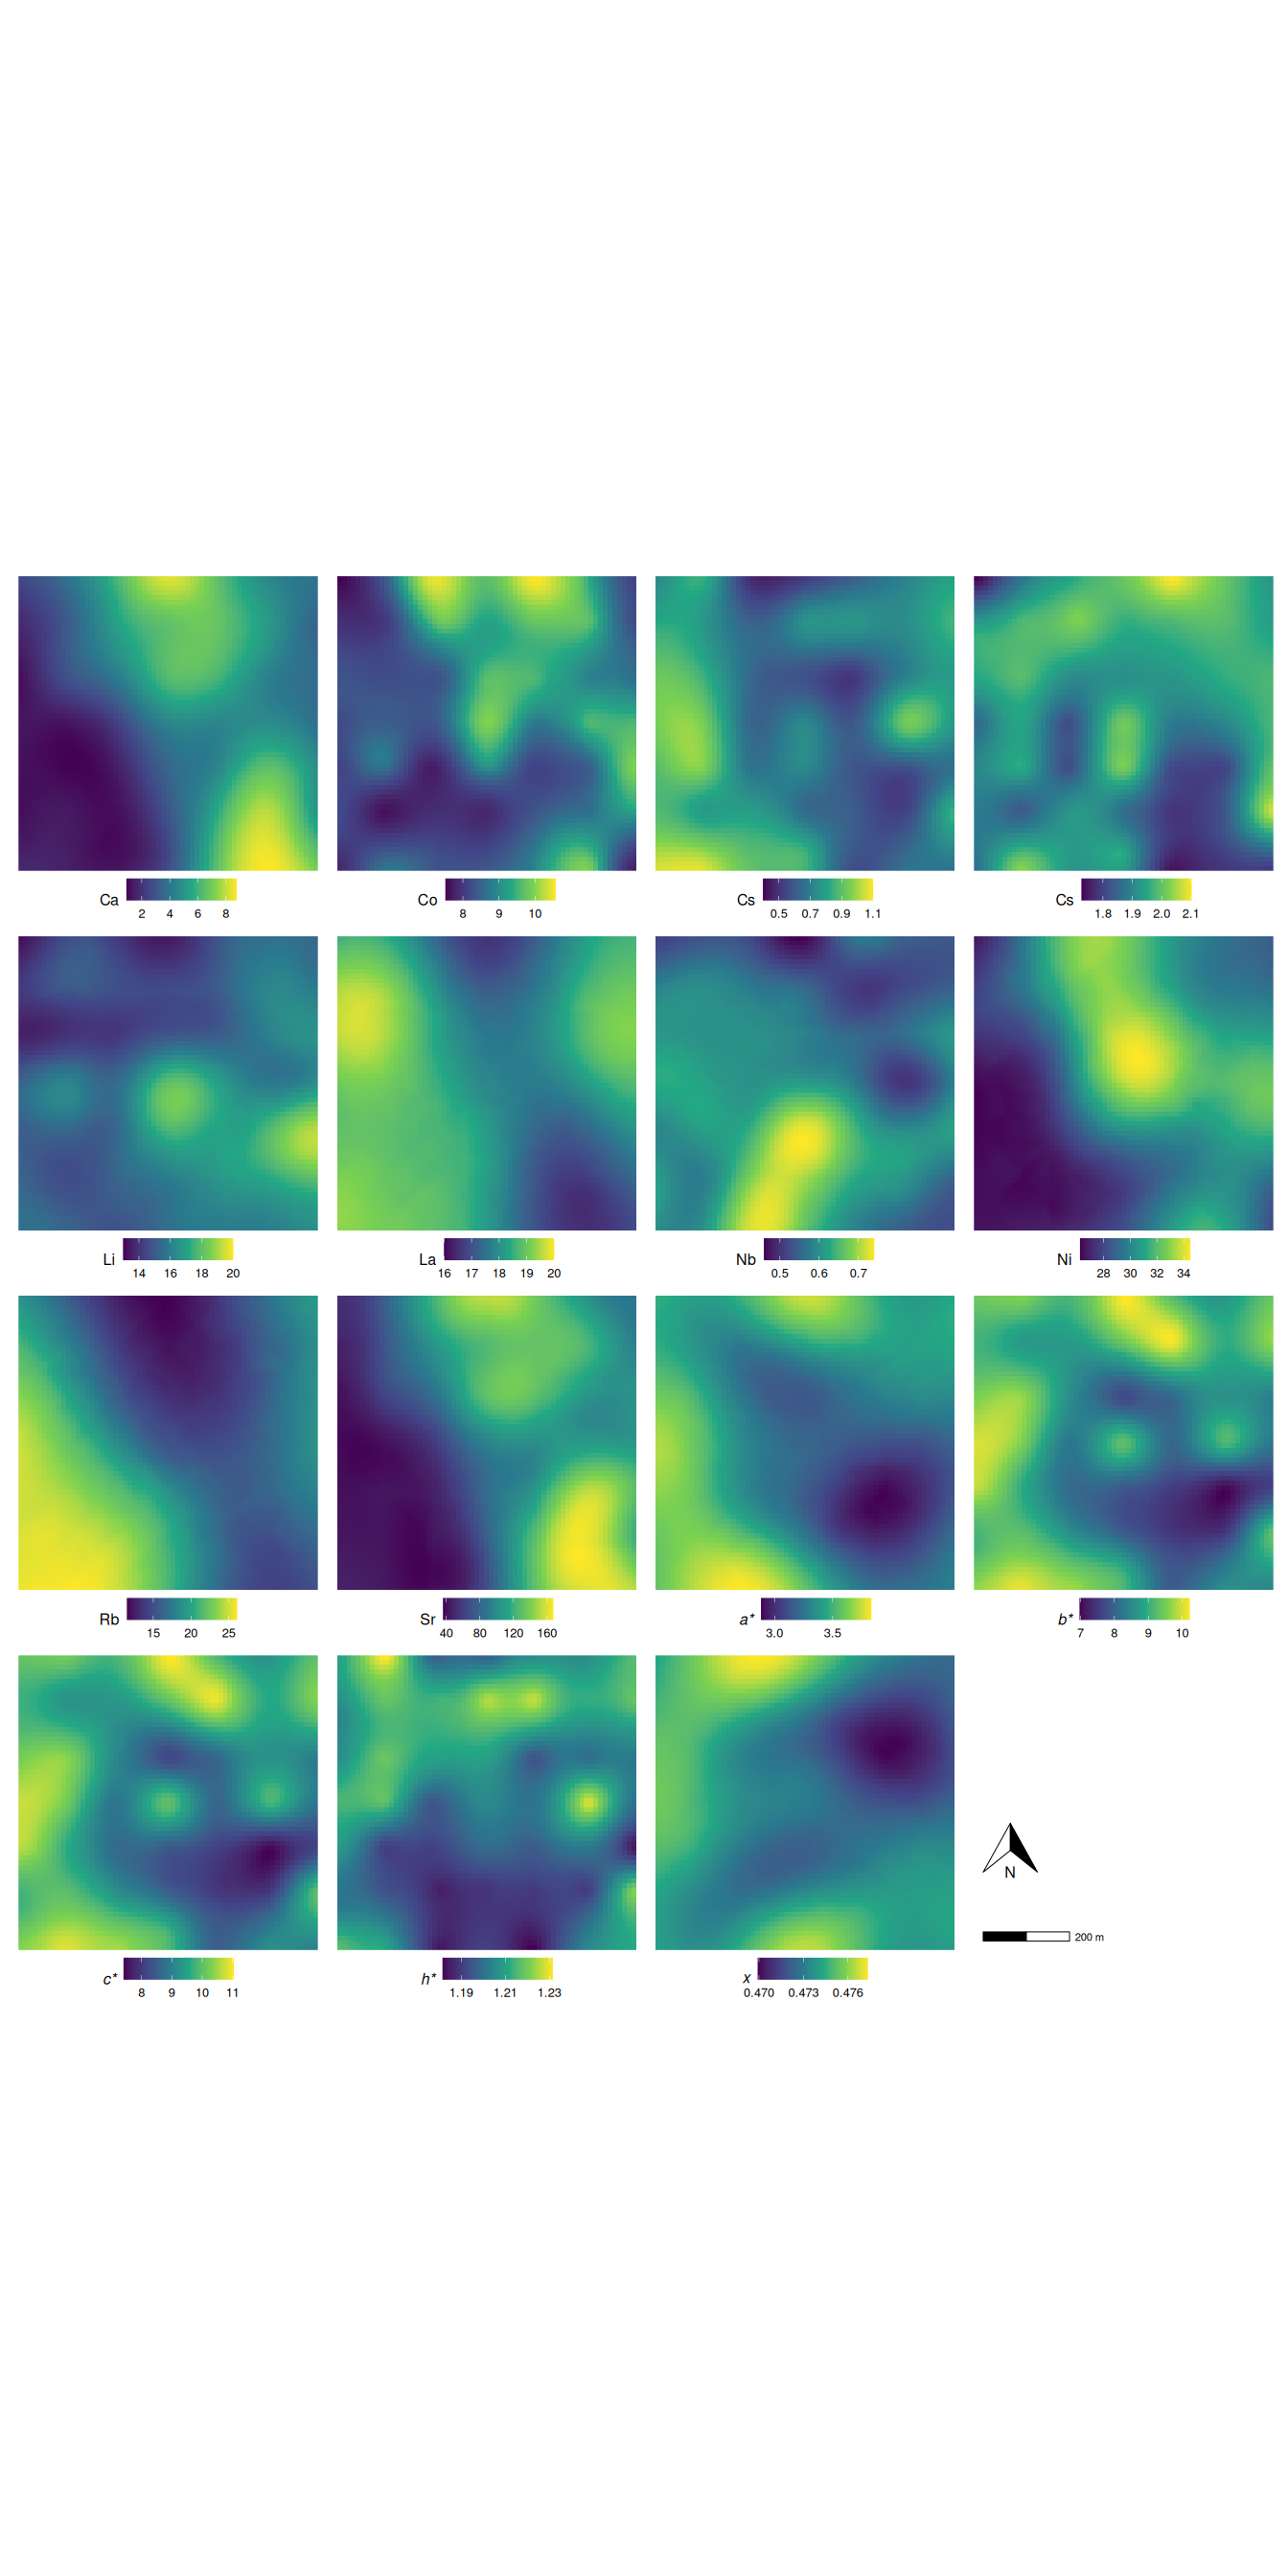
\includegraphics[keepaspectratio]{index_files/figure-latex/notebooks-property_maps-fig-ag_map-output-1.png}}

}

\caption{\label{fig-ag_map}Kriged maps of select colour and geochemical
properties and elevation across the agricultural site.}

\end{figure}%

\textsubscript{Source:
\href{https://alex-koiter.github.io/terrain-attributes/notebooks/property_maps.qmd.html\#cell-fig-ag_map}{Soil
property mapping}}

\begin{figure}[H]

\centering{

\pandocbounded{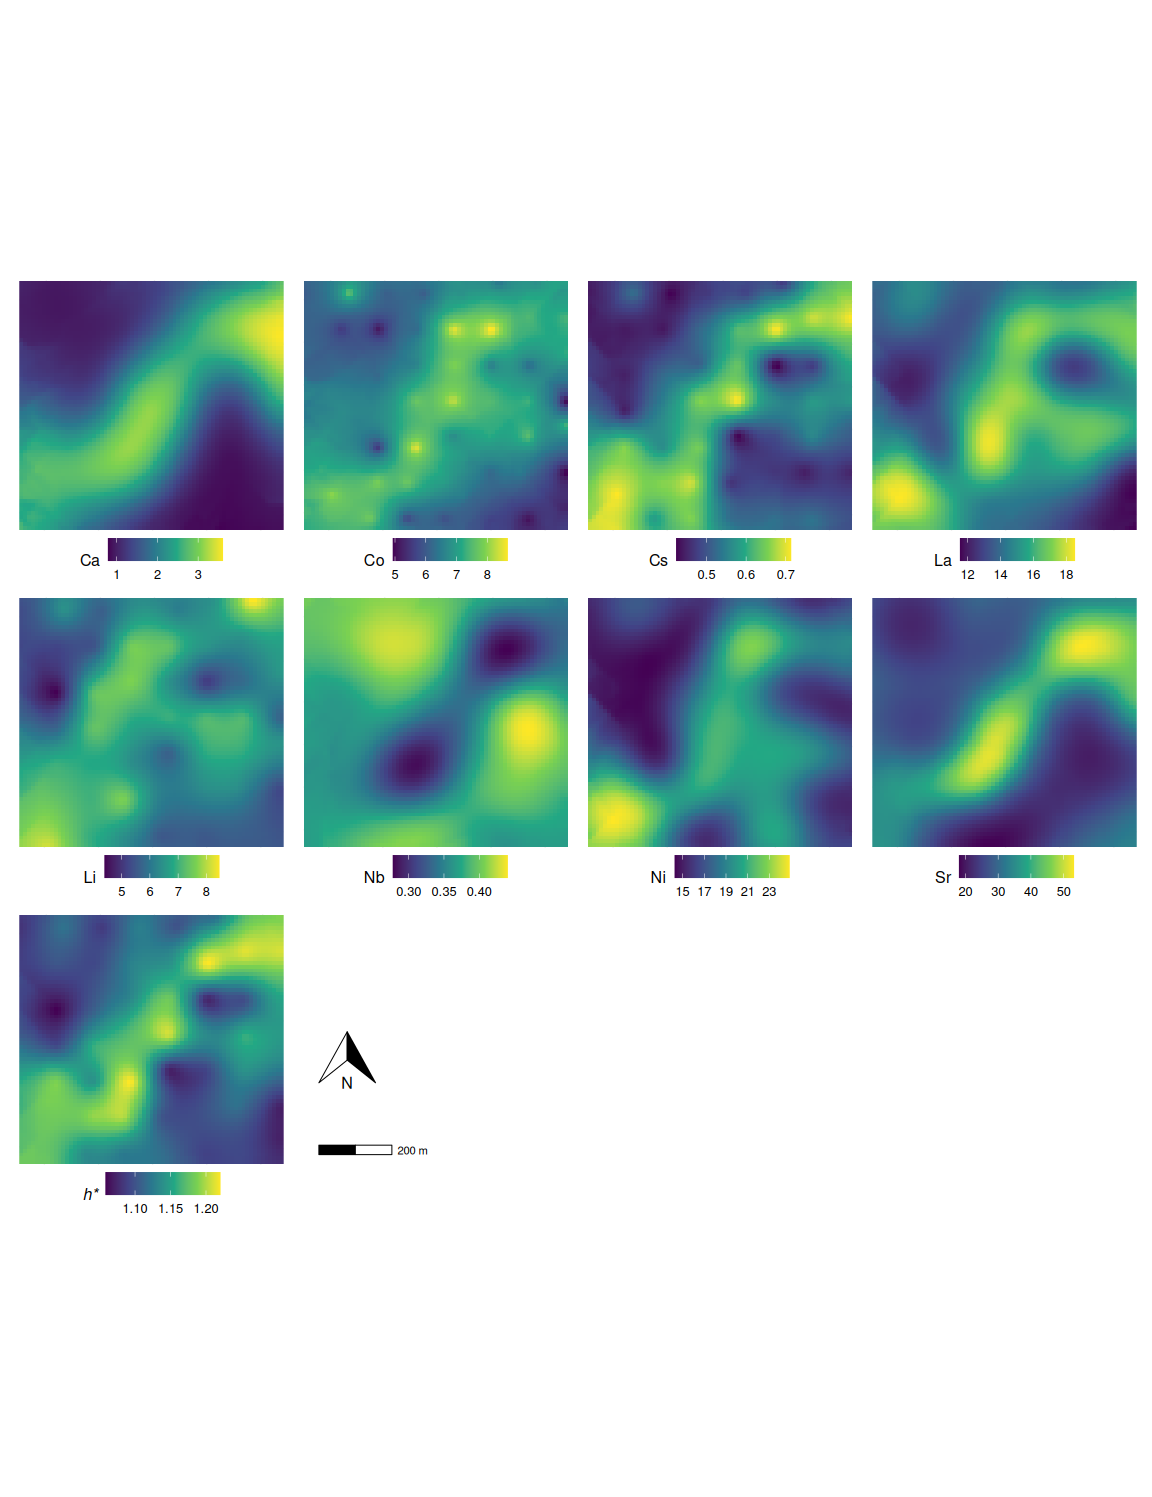
\includegraphics[keepaspectratio]{index_files/figure-latex/notebooks-property_maps-fig-forest_map-output-1.png}}

}

\caption{\label{fig-forest_map}Kriged map of select colour and
geochemical properties and elevation across the forested site.}

\end{figure}%

\textsubscript{Source:
\href{https://alex-koiter.github.io/terrain-attributes/notebooks/property_maps.qmd.html\#cell-fig-forest_map}{Soil
property mapping}}

With the exception of \emph{h*} all the soil properties measured at the
agricultural site were significantly (p \textless{} 0.05) correlated
with the elevation and the wetness index (Table~\ref{tbl-correlation}).
A few soil properties (Li, Ni, Sr, \emph{a*} and \emph{x*}) were
correlated relative slope position and vertical distance to the channel,
and there was little to no correlation with catchment area and curvature
attributes. Overall there was little correlation between soil properties
and terrain attributes at the forested site
(Table~\ref{tbl-correlation}).

\begin{longtable}[]{@{}cccccccc@{}}

\caption{\label{tbl-correlation}Pearson's correlation coefficients for
select soil properties and terrain attributes (n=49).}

\tabularnewline

\toprule\noalign{}
Property & Elevation & SAGA Wetness Index & Rel. Slope Position & Vert.
Dist. Channel & Catchment Area & Plan Curvature & Profile Curvature \\
\midrule\noalign{}
\endhead
\midrule\noalign{}
\multicolumn{8}{@{}c@{}}{%
*** p \textless{} 0.001; ** p \textless{} 0.01; * p \textless{} 0.05; NS
= non-significant at p = 0.05} \\
\bottomrule\noalign{}
\endlastfoot
\multicolumn{8}{@{}c@{}}{%
Agriculture} \\
{Ca} & -0.71*** & 0.61*** & NS & -0.32* & NS & NS & NS \\
{Co} & -0.52*** & 0.56*** & NS & NS & NS & NS & NS \\
{Cs} & 0.56*** & -0.5*** & NS & NS & NS & NS & NS \\
{Fe} & NS & 0.33* & NS & NS & NS & NS & NS \\
{Li} & -0.39** & 0.38** & -0.56*** & -0.39** & NS & NS & NS \\
{La} & 0.51*** & -0.39** & NS & NS & NS & NS & NS \\
{Nb} & 0.41** & -0.41** & NS & NS & NS & NS & NS \\
{Ni} & -0.72*** & 0.73*** & -0.29* & -0.32* & NS & NS & NS \\
{Rb} & 0.78*** & -0.72*** & NS & 0.32* & NS & NS & NS \\
{Sr} & -0.78*** & 0.7*** & -0.39** & -0.38** & NS & NS & NS \\
{*a**} & 0.6*** & -0.49*** & 0.43** & 0.36* & NS & NS & NS \\
{*b**} & 0.39** & -0.31* & NS & NS & NS & NS & NS \\
{*c**} & 0.4** & -0.31* & NS & NS & NS & NS & NS \\
{*h**} & NS & NS & NS & NS & NS & NS & -0.3* \\
{\emph{x}} & 0.48*** & -0.55*** & 0.5*** & 0.41** & -0.37** & NS & NS \\
\multicolumn{8}{@{}c@{}}{%
Forest} \\
{Ca} & NS & -0.58*** & NS & 0.45** & 0.35* & NS & NS \\
{Co} & NS & NS & NS & NS & NS & NS & NS \\
{Cs} & NS & NS & NS & NS & 0.33* & NS & NS \\
{Li} & NS & NS & NS & NS & NS & NS & NS \\
{La} & NS & NS & NS & NS & NS & NS & NS \\
{Nb} & NS & 0.57*** & NS & -0.45** & NS & NS & NS \\
{Ni} & NS & NS & NS & NS & NS & NS & NS \\
{Sr} & -0.35* & -0.58*** & NS & 0.44** & 0.31* & NS & NS \\
{*h**} & NS & NS & NS & 0.31* & 0.33* & NS & NS \\

\end{longtable}

\textsubscript{Source:
\href{https://alex-koiter.github.io/terrain-attributes/notebooks/univariate_analysis.qmd.html\#cell-tbl-correlation}{Univariate
summary}}

No multicollinearity among the terrain attributes at either site was
detected and all seven attributes were retained for all analysis. The
mtry parameter selected for each model varied with most using a value of
four. The RF regression model showed variable explanatory power and
performance across soil properties and sites
(Table~\ref{tbl-rf-summary}). For the agriculture site, the model
explained a low to moderate proportion of variance, ranging from 17.2\%
(Nb) to 76.1\% (Rb). Interestingly the RF analysis for Li yielded a
negative percent variation explained the suggesting that using the
average value is a better predictor. Testing the model showed moderately
good to poor performance with r\textsuperscript{2} values ranging from
0.01 (Fe) to 0.85 (Rb, Sr). The SAGA Wetness Index and elevation were
generally the most important terrain attributes in the model with
profile and plan curvature as the least important terrain attributes
(Figure~\ref{fig-rf-results}). Additional details on variable importance
are provided in \quartosuppfigref{suppfig-ag_RF_summary}.

\begin{longtable}[]{@{}
  >{\centering\arraybackslash}p{(\linewidth - 8\tabcolsep) * \real{0.2000}}
  >{\centering\arraybackslash}p{(\linewidth - 8\tabcolsep) * \real{0.2000}}
  >{\centering\arraybackslash}p{(\linewidth - 8\tabcolsep) * \real{0.2000}}
  >{\centering\arraybackslash}p{(\linewidth - 8\tabcolsep) * \real{0.2000}}
  >{\centering\arraybackslash}p{(\linewidth - 8\tabcolsep) * \real{0.2000}}@{}}

\caption{\label{tbl-rf-summary}Model summary and performance statistics
for the random forest regression using the training and test data sets.}

\tabularnewline

\toprule\noalign{}
\multirow{2}{=}{\begin{minipage}[b]{\linewidth}\raggedright
Property
\end{minipage}} &
\multicolumn{2}{>{\centering\arraybackslash}p{(\linewidth - 8\tabcolsep) * \real{0.4000} + 2\tabcolsep}}{%
\begin{minipage}[b]{\linewidth}\centering
Training
\end{minipage}} &
\multicolumn{2}{>{\centering\arraybackslash}p{(\linewidth - 8\tabcolsep) * \real{0.4000} + 2\tabcolsep}@{}}{%
\begin{minipage}[b]{\linewidth}\centering
Test
\end{minipage}} \\
& \begin{minipage}[b]{\linewidth}\raggedright
\% Variance{\textsuperscript{1}}
\end{minipage} & \begin{minipage}[b]{\linewidth}\raggedright
MSE{\textsuperscript{2}}
\end{minipage} & \begin{minipage}[b]{\linewidth}\raggedright
r{\textsuperscript{2}}
\end{minipage} & \begin{minipage}[b]{\linewidth}\raggedright
MSE{\textsuperscript{2}}
\end{minipage} \\
\midrule\noalign{}
\endhead
\midrule\noalign{}
\multicolumn{5}{@{}>{\centering\arraybackslash}p{(\linewidth - 8\tabcolsep) * \real{1.0000} + 8\tabcolsep}@{}}{%
{\textsuperscript{1}} Percent variance explained} \\
\multicolumn{5}{@{}>{\centering\arraybackslash}p{(\linewidth - 8\tabcolsep) * \real{1.0000} + 8\tabcolsep}@{}}{%
{\textsuperscript{2}} Mean square error} \\
\bottomrule\noalign{}
\endlastfoot
\multicolumn{5}{@{}>{\centering\arraybackslash}p{(\linewidth - 8\tabcolsep) * \real{1.0000} + 8\tabcolsep}@{}}{%
Agriculture} \\
Co & 33.2 & 0.43 & 0.11 & 0.51 \\
Cs & 57.4 & 0.01 & 0.29 & 0.01 \\
Fe & 34.4 & 0.01 & 0.01 & 0.01 \\
Li & −14.9 & 1.86 & 0.43 & 0.84 \\
La & 37.4 & 0.39 & 0.81 & 0.38 \\
Nb & 17.2 & 0.00 & 0.00 & 0.00 \\
Ni & 65.1 & 1.89 & 0.70 & 1.46 \\
Rb & 76.1 & 3.75 & 0.85 & 2.71 \\
Sr & 64.4 & 441.33 & 0.85 & 365.51 \\
a* & 41.5 & 0.03 & 0.48 & 0.02 \\
b* & 31.8 & 0.53 & 0.09 & 0.40 \\
c* & 29.2 & 0.64 & 0.10 & 0.49 \\
h* & 20.2 & 0.00 & 0.03 & 0.00 \\
x & 34.5 & 0.00 & 0.31 & 0.00 \\
\multicolumn{5}{@{}>{\centering\arraybackslash}p{(\linewidth - 8\tabcolsep) * \real{1.0000} + 8\tabcolsep}@{}}{%
Forest} \\
Ca & 41.5 & 0.32 & 0.25 & 0.58 \\
Co & −17.3 & 0.97 & 0.01 & 1.03 \\
Cs & −5.6 & 0.01 & 0.02 & 0.01 \\
Li & −8.1 & 0.55 & 0.05 & 1.33 \\
La & −31.2 & 2.49 & 0.02 & 3.77 \\
Nb & 36.1 & 0.00 & 0.16 & 0.00 \\
Ni & −43.7 & 7.78 & 0.02 & 6.98 \\
Sr & 40.1 & 44.47 & 0.17 & 58.18 \\
h* & −13.7 & 0.00 & 0.01 & 0.00 \\

\end{longtable}

\textsubscript{Source:
\href{https://alex-koiter.github.io/terrain-attributes/notebooks/RF_summary.qmd.html\#cell-tbl-rf-summary}{Random
Forest summary}}

\begin{figure}[H]

\centering{

\pandocbounded{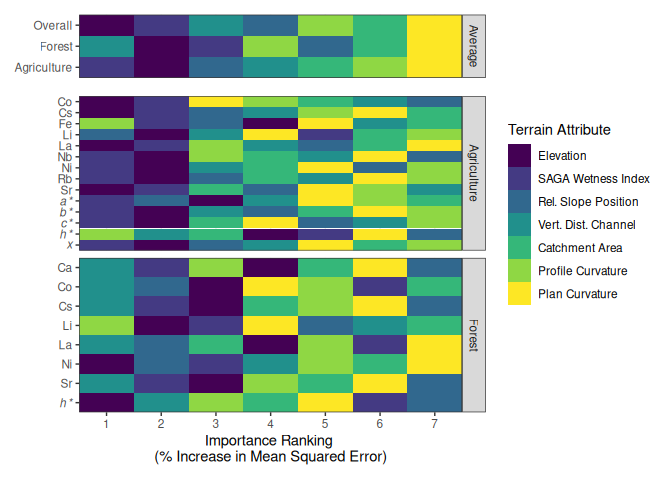
\includegraphics[keepaspectratio]{index_files/figure-latex/notebooks-RF_summary-fig-rf-results-output-1.png}}

}

\caption{\label{fig-rf-results}Heat map of the Random Forest regression
results showing the ranking of the importance of terrain attributes
(based on \% increase in Mean Squared Error) in explaining the spatial
variabilty of selected colour and geochemical properties within the
agricultural and forested sites. Top panel shows an average ranking for
each site and across both sites.}

\end{figure}%

\textsubscript{Source:
\href{https://alex-koiter.github.io/terrain-attributes/notebooks/RF_summary.qmd.html\#cell-fig-rf-results}{Random
Forest summary}}

Overall the RF regression analysis at the forested site demonstrated
poor explanatory power and low performance (Table~\ref{tbl-rf-summary}).
The RF models for Ca, Nb, and Sr explained a moderate proportion of
variance. Similar to Li at the agricultural site, all other soil
properties demonstrated that the average value was a better predictor.
Model performance was also poor with all r\textsuperscript{2} values
below 0.2. The importance ranking varied considerably between soil
properties; however, the vertical distance to channel and elevations
were generally the most important terrain attributes in the model
(Figure~\ref{fig-rf-results}).

\subsection{Discussion}\label{discussion}

\subsubsection{Variability of soil
properties}\label{variability-of-soil-properties}

Variability in soil geochemical properties has been studied at a range
of scales including continental (Drew et al., 2010), regional
(Rattenbury et al., 2018), watershed (Nanos and Rodríguez Martín, 2012),
hillslope/catena, and farm field (Sun et al., 2021b). The objectives of
these studies included addressing issues of pollution/contamination,
providing benchmark/baseline information, investigating pedological and
weathering properties and processes, and soil surveying and mapping
(Wilson et al., 2008). Variability in soil colour, typically using the
Munsell colour system, is a commonly reported diagnostic feature used in
soil classification and ranges in spatial scales from reconnaissance to
detailed soil surveys and maps. For sediment fingerprinting studies,
these types of studies are often too site-specific or focus on a smaller
subset of soil properties to effectively guide sample design to ensure
the desired confidence is met characterizing sources of sediment. Data
distributions in soil science commonly exhibit a positively skewed
distribution. This is likely due to several factors including that data
of this nature are a semi-bounded distribution, with a lower bound of
zero and no upper bound. Hot spots of soil processes, local variations
in soil forming factors, and soil/land management practices can also
lead to more extreme values (e.g., Vidon et al., 2010). In many cases
the cumulative effects of these processes, factors, and practices are
multiplicative (i.e., interact) and not linearly additive, resulting in
a skewed data distribution. Lastly, the distribution of data will also
be a product of the scale of observation, number of samples, and
sampling design. Soil colour properties exhibited a near-normal
distribution with a low CV which is consistent with claims that soil hue
and value (Munsell colour system) have a low CV (Pennock et al., 2008).
These data distribution properties are ideal for statistical and
environmental modeling as it typically meets the model assumptions with
out requiring transformations. Soil colour coefficients (*a**, *b**,
*c**, *h**, x) showed near-normal distributions and low CVs (Table~1),
supporting their suitability for mixing models that assume normality and
require low within-source variability.

The geochemical properties exhibited greater variability and skewness
despite removing coarse fraction, reflecting site-specific pedogenic and
geomorphic processes and organic matter differences. Trace elements
correlate strongly with fine material (\textless2 μm) due to its high
surface area and reactivity (Horowitz, 1991). Removing sand-sized
material reduced grain-size effects, likely resulting in lower
variability than in bulk soil studies (\textless2 mm). In particular,
the forest site exhibited a greater amount of variability which is
likely due to the more complex topography and geomorphic setting. The
floodplain within the forested site is likely accumulating shale-rich
material derived from the Manitoba Escarpment which is enriched in trace
metals (Nicolas and Bamburak, 2011). This creates a zone of high
concentrations relative to upland areas (Figure~\ref{fig-forest_map}).
The forested site also had a higher and much more variable soil organic
matter content (x̄ = 8.5 \%, CV = 51.9 \%) as compared to the
agricultural site (x̄ = 11.6 \%, CV = 16.1 \%), which similarly to the
grain size distribution, can influence the concentration of many major
and trace elements (Horowitz, 1991). These results provide evidence that
land use and landscape complexity play a role in driving soil property
variability that can be considered when developing a strategic sampling
design.

\subsubsection{Spatial distribution}\label{spatial-distribution}

The difference in the number of soil properties and the magnitude of the
spatial auto correlation between the two sites can be used in designing
an effect sampling campaign. The agricultural site, which has a simpler
topography and a higher degree of spatial autocorrelation, grid sampling
with spacing on the order of the semivariogram range (∼200--220 m) is
adequate for mapping. In contrast, the forested site, which has a more
complex geomorphic setting and a lower degree of spatial
autocorrelation, a stratified sampling design is recommended. At the
forested site the stratas could include near-stream and hillslope
environments. When the spatial distribution of soil properties are
unknown, often the case in fingerprinting studies, it is recommended
that sampling include irregularly spaced points (including \textless100
m) to better resolve short-range structure. This is important for
improving variogram modeling and kriging interpolation (Lark and
Marchant, 2018). Properties lacking spatial autocorrelation at the
forest site (Fe, Rb, \emph{a*, b*}, c*, x) likely reflect mixed
depositional environments and fine-scale heterogeneity that exceed the
sampling resolution; acknowledging their behavior is critical when
selecting fingerprints.

Mapping the soil properties that have a moderate to high spatial
dependence can provide information on underlying soil forming processes
and properties. At both sites, to some extent, the patterns appear to
reflect the topography of the sites suggesting that geomorphic and
hydrologic processes and properties are likely driving the observed
patterns. Koiter et al.~(2013) discussed the issues surrounding the use
of a statistical only approach to selecting fingerprints and that
consideration of how fingerprints have developed improves the robustness
of the sediment fingerprinting approach. However, local information on
the spatial distribution of geochemical and colour properties at field
scales (\textless{} 1 km²) is often unavailable, and the processes
driving these patterns are also not well documented or studied. When
such information does exist, it typically focuses on agronomically
important properties (e.g., Mzuku et al., 2005) or is used for soil
classification (e.g., Soil Classification Working Group, 1998). These
datasets usually include geochemical properties such as N, P, K, S, Ca,
Mg, Na, Fe, and Al. They may also include colour characteristics, such
as Munsell hue, value, and chroma, as well as other soil properties like
texture, organic matter content, and pH. The lack of information on the
wide range of soil properties used in fingerprinting studies means the
researchers are relying on other data, most often elevation and
geomorphic/topographic features, for informing sampling designs. The
results from this study support this approach.

\subsubsection{Terrain attributes and soil
properties}\label{terrain-attributes-and-soil-properties}

The correlation analysis identified elevation and wetness as being
significantly correlated to most of the fingerprint properties at the
agricultural site. Similarly, the RF regression identified elevation,
wetness, and relative slope position as important attributes in
explaining most of the observed variation in soil geochemical and colour
properties. These terrain attributes align with established pedogenic
and geomorphic processes, including eluviation--illuviation of Fe and
clay, carbonate dissolution and transport, and organic matter
accumulation in lower positions, and thereby indirectly influence soil
geochemistry and colour. The results of this study are consistent with
the findings of Mashalaba et al.~(2020) who also found that similar
terrain attributes were important in predicting a range of other soil
properties including texture, bulk density, and hydaulic conductivity.
These attributes likely emerged as the most important factor in
explaining the observed variability as they are strongly linked to a
range of geomorphic and hydrologic process and conditions (Libohova et
al., 2024; Mello et al., 2022). For example, in eroded landscapes in the
Prairie region of Canada, Ca concentrations have been found to be higher
in upper slope positions from erosion and subsequent exposure of
high-carbonate subsoil (Papiernik et al., 2005). In contrast, higher Ca
concentrations have been noted in lower slope and depressional areas due
to higher solubility of many Ca-minerals (e.g., CaCO3) and the
subsequent downslope transport in solution and reduced leaching losses
in these accumulation zones. Landscape position can also have a strong
influence on pedogenic process; for example, the translocation of Fe and
clay down the soil profile is a diagnostic criteria used in classifying
soils (Stonehouse and St.~Arnaud, 1971). Soil colour also tends to
change in a predictable manner in relation to local relief. Tillage and
water erosion results in the net loss of darker organic-rich topsoil
from upper slope positions resulting in the exposure of the lighter
subsoil (Papiernik et al., 2005). Moisture availability is also greater
in the lower slope and depressional areas resulting in increased organic
matter production resulting in darker organic-rich topsoil as compared
to the upper slope positions. There is also evidence that suggests that
soil texture varies with elevation and slope position, with coarser
material on upper slopes and finer material accumulating in lower
positions (Cox et al., 2003; Kokulan et al., 2018). Given the strong
correlation of organic matter and texture with soil geochemistry
(Horowitz, 1991) and colour (Viscarra Rossel et al., 2009), these
properties may also help explain the observed spatial patterns .
Compared to the forest site, the RF regression model showed greater
explanatory power and predictive performance for the agricultural site,
likely due to its simpler topography. In these settings, terrain
attributes can serve as an initial step in developing efficient and
effective sampling designs (Pham et al.~2025). As high-quality LiDAR
data and digital elevation models (DEMs) become increasingly available
in many regions, researchers have the opportunity to integrate terrain
attributes into their sampling frameworks. This integration ensures
adequate representation of key geomorphic and topographic features.
However, at the forested site, the RF model showed poor fit, and terrain
variables were largely uninformative; this likely reflects the increased
geomorphic complexity of the site and the limitations of sparse
sampling. Additional work is needed to fully assess the utility of
terrain mapping in predicting and mapping fingerprint properties,
particularly in complex terrains.

\subsubsection{Limitations and Future
Work}\label{limitations-and-future-work}

The impact of sampling design the characterization of fingerprints can
be substantial (Luna Miño et al., 2024), which in turn can affect the
apportionment results, and the conclusion and recommendations drawn from
them. However, due to the high cost of sample collection, preparation,
and analysis, small sample sizes collected across a single season are
commonplace and a source of uncertainty in sediment fingerprinting
studies (Evrard et al.~2022). Therefore, the development of low-cost,
easy, and accurate mapping of fingerprinting properties would be
advantageous. Terrain attributes have been successfully used in digital
soil mapping exercises, demonstrating their value in spatially
characterizing soil properties (Rizzo et al.~2016). Building on this
success, integrating terrain analysis into sediment source
fingerprinting is promising, not only as a mechanism to improve the
quality of source characterization, but to also better link source
material to downstream sediment. However, the inclusion of only two
sites within in this study limits the generalizability of the findings
to geomorphic settings with similar characteristics, highlighting the
need for future research across a broader range of environments.

The relatively small sample size (n=49 per site) in this study
compromises the stability of the RF-derived importance metrics.
Similarly, the 100 m sample spacing likely misses fine-scale
heterogeneity limiting the semivariogram models ability to capture
short-range spatial variability. As a result, additional sampling at
irregular spacing is highly recommended. Because this study relies on
single season of sampling there is no information on the stability of
soil properties over time. While sediment fingerprinting assumes
consistent source signatures over time, few studies validate this due to
the challenges associated with repeated sample collection (Evrard et
al.~2022).

The continued integration of DEM-based sampling strategies and
fingerprint mapping into sediment source fingerprinting approach will
benefit from the development of a standardized framework, workflow, and
set of best practices to ensure both robust and reliable results. For
example, differences in DEM resolution between sites in this study could
influence curvature-based terrain attributes, introducing potential
bias. Furthermore, the use of isotropic variogram models may not
adequately represent spatial autocorrelation in channelized landscapes,
where directional variability is expected. Additional work is needed to
establish standardized protocols for DEM processing, terrain attribute
calculation, and variogram modeling to ensure that methods work across a
range of landscapes.

\subsection{Conclusions}\label{conclusions}

Understanding the spatial variability and distribution of soil
geochemical and colour properties at a field-scale is an important part
of sediment source fingerprinting. This study conducted both univariate
and spatial analyses of a suite of soil geochemical and colour
properties at two sites with contrasting land uses. The agricultural
site, characterized by a simple topography, exhibited lower coefficients
of variation, approximately normal data distributions, and moderate to
strong spatial autocorrelation across most measured properties. In
contrast, the forested site featured more geomorphologically complex
terrain, with greater variability in soil properties, data distributions
that more frequently deviated from normality, and fewer properties
exhibiting spatial autocorrelation. Random forest regression
demonstrated that many fingerprint-relevant properties exhibit usable
spatial dependence at the field scale and are structured by terrain
attributes. Elevation, wetness, and slope position explained a
substantial portion of the observed variability, ssupporting the use of
DEM-guided sampling strategies. For effective mapping of sediment
fingerprinting properties at the field scale, a grid spacing
approximately equal to the site-specific semivariogram range
(\textasciitilde200--230 m) is recommended. In areas with complex
terrain, stratified sampling should be implemented to capture spatial
variability and improve representativeness. Furthermore, colour
coefficients such as \emph{a*, b*, c*, h*}, and \emph{x} are ideal for
inclusion in sediment mixing models when low coefficients of variation
and near-normal data distributions are assumed.

\subsection*{Acknowledgments}\label{acknowledgments}
\addcontentsline{toc}{subsection}{Acknowledgments}

Special thanks and recognition for the field and technical support from
A. Avila and the Riding Mountain National Park personnel.

\subsection*{Statements and
declarations}\label{statements-and-declarations}
\addcontentsline{toc}{subsection}{Statements and declarations}

\subsubsection*{Funding}\label{funding}
\addcontentsline{toc}{subsubsection}{Funding}

This research was supported by the Natural Sciences and Engineering
Research Council of Canada Discovery Grant - From source to sink:
Investigating the linkages between sources of sediment and downstream
water quality in Canadian watersheds - awarded to AJK
(RGPIN-2019-05273).

\subsubsection*{Competing interests}\label{competing-interests}
\addcontentsline{toc}{subsubsection}{Competing interests}

The authors have no competing interests to declare that are relevant to
the content of this article.

\subsubsection*{Data and code
availability}\label{data-and-code-availability}
\addcontentsline{toc}{subsubsection}{Data and code availability}

Data and source code for analysis and manuscript available on GitHub:
\url{https://github.com/alex-koiter/sampling-design-manuscript}

\subsubsection*{Author contributions}\label{author-contributions}
\addcontentsline{toc}{subsubsection}{Author contributions}

\textbf{M Luna Miño} Methodology; Investigation; Data curation; Formal
analysis; Writing - Original Draft; Writing - Review \& Editing

\textbf{A Koiter}: Conceptualization; Funding acquisition; Methodology;
Investigation; Data curation; Formal analysis; Visualization; Writing -
Original Draft; Writing -- review and editing; Software; Project
administration

\textbf{T Lychuk}: Methodology; Formal analysis; Writing - Review \&
Editing

\textbf{A Waddel} Methodology; Formal analysis; Writing - Review \&
Editing

\textbf{A Moulin} Methodology; Formal analysis; Writing - Review \&
Editing

\subsection*{References}\label{references}
\addcontentsline{toc}{subsection}{References}

\renewcommand{\bibsection}{}
\bibliography{references.bib}

\subsection{Supplemental figures}\label{supplemental-figures}

\begin{suppfig}

\centering{

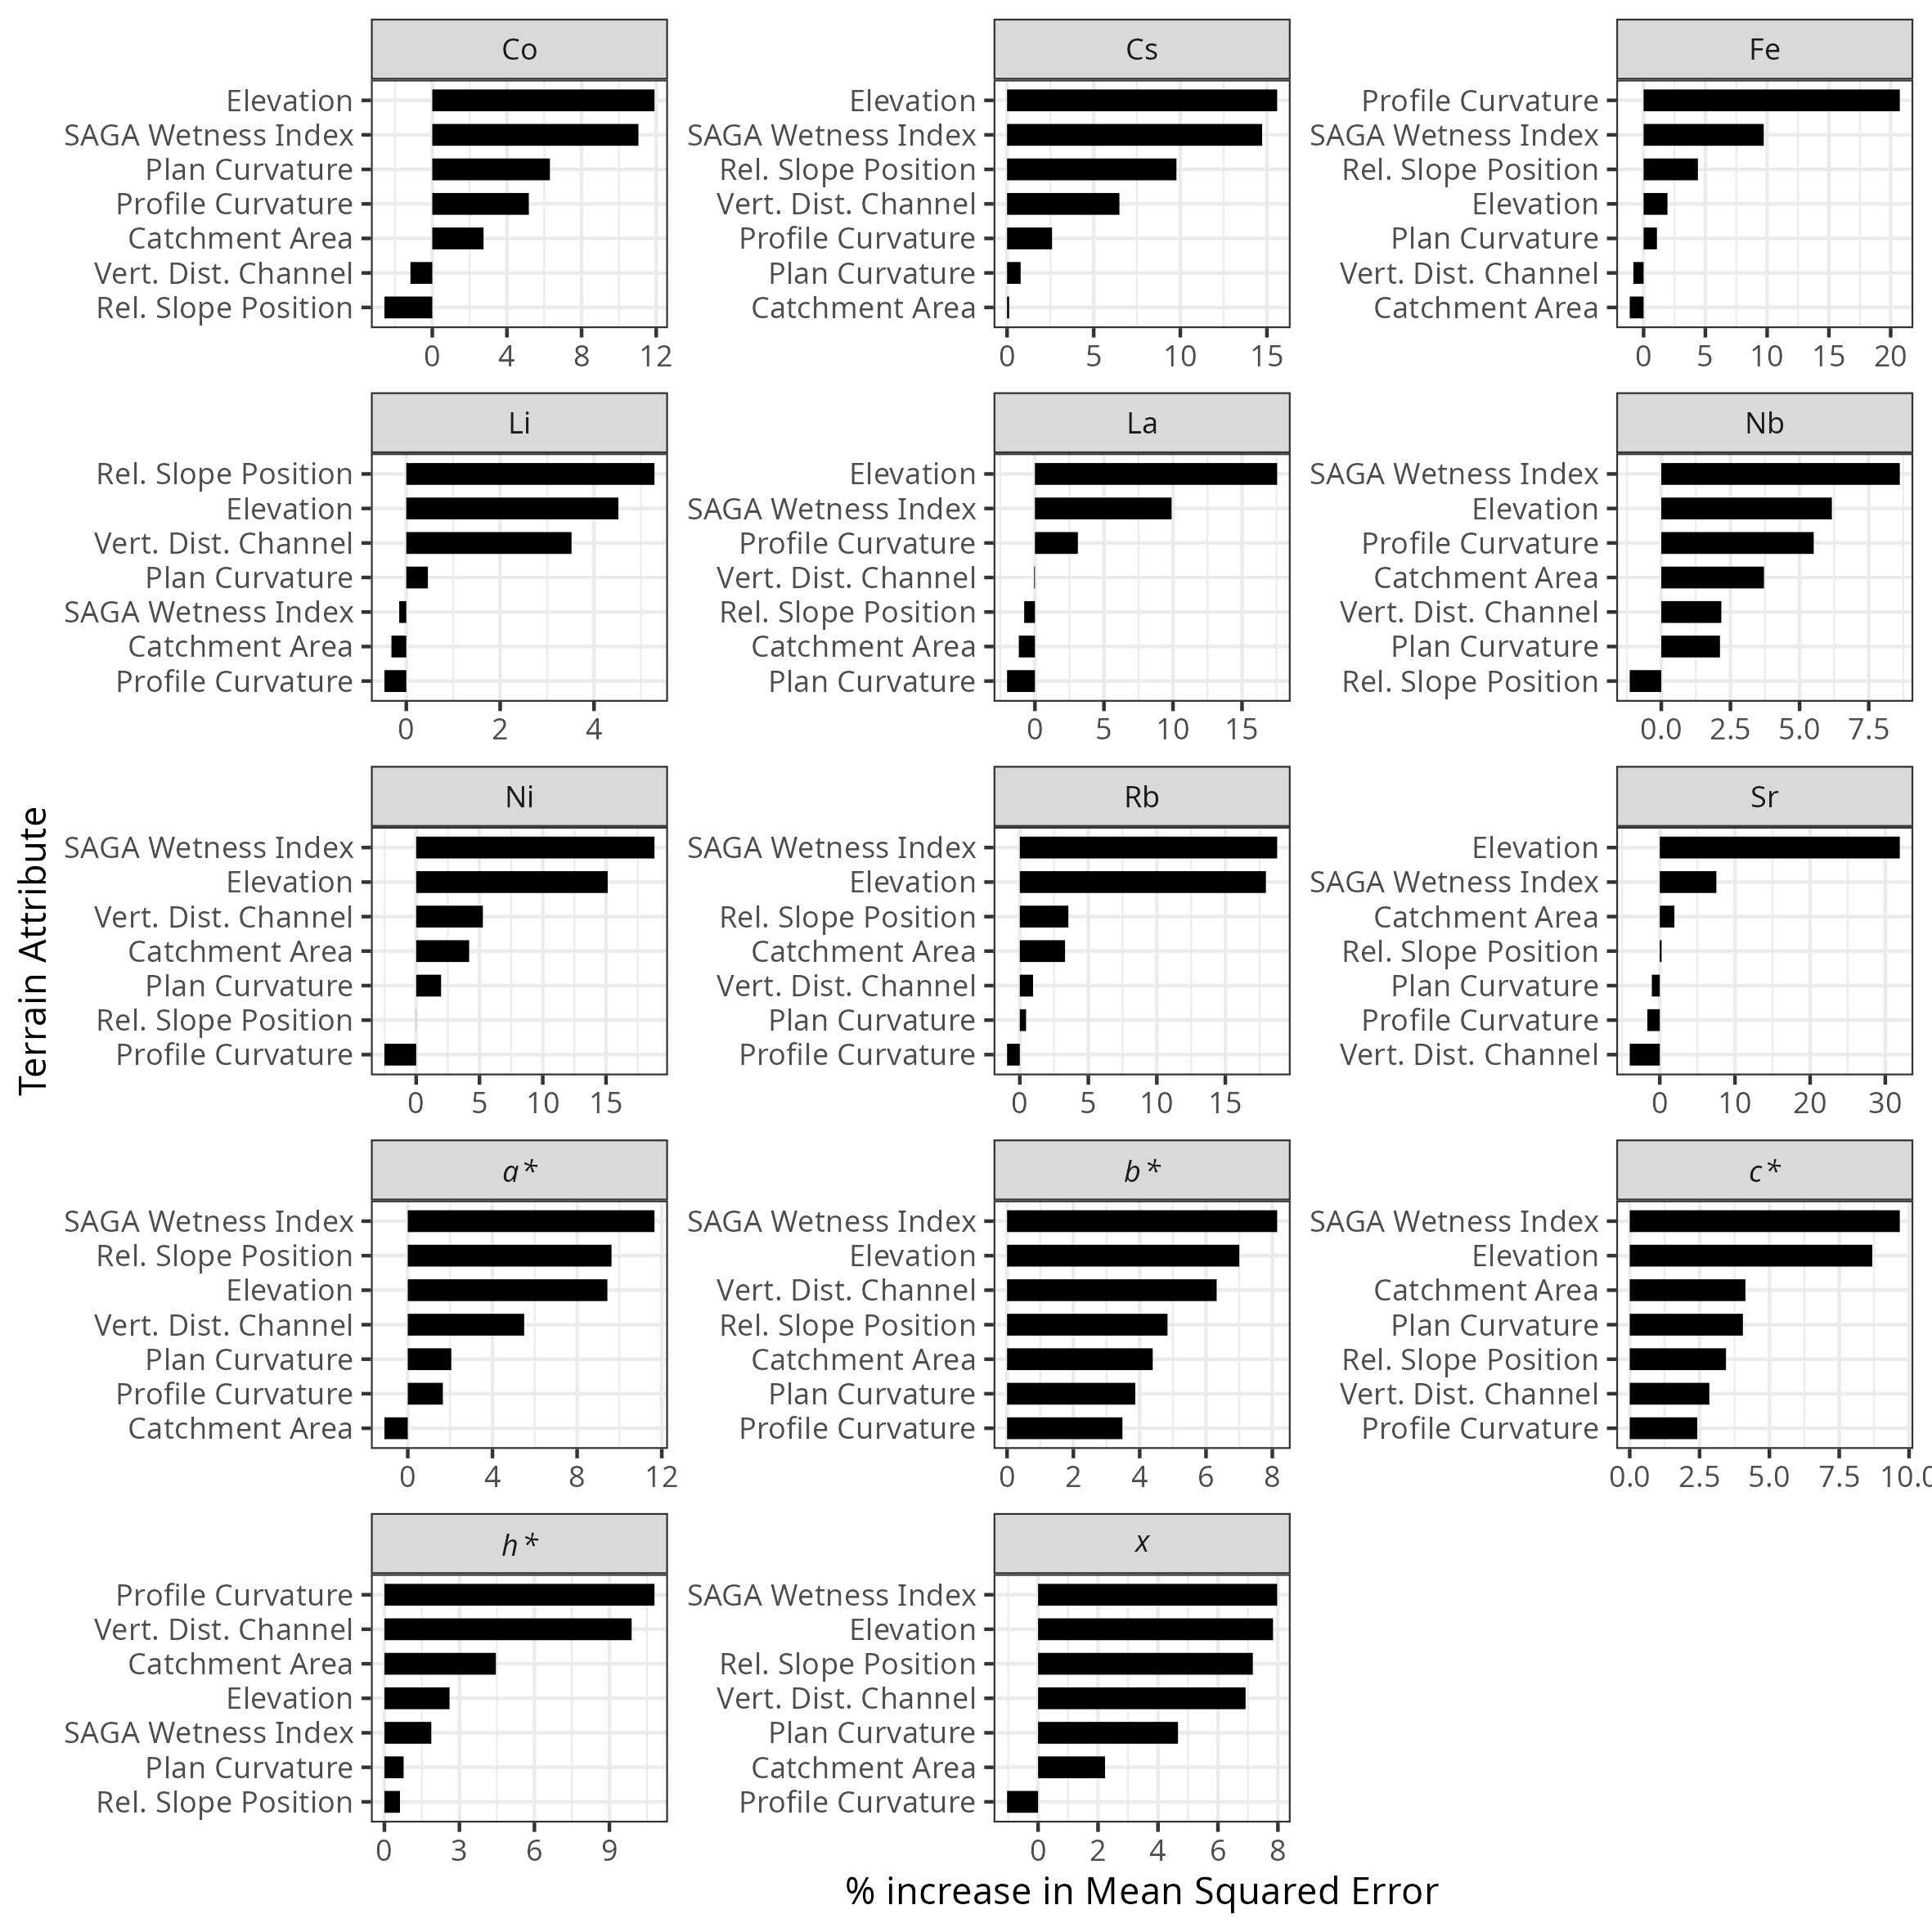
\includegraphics[width=1\linewidth,height=\textheight,keepaspectratio]{images/Ag_RF_summary.png}

}

\caption{\label{suppfig-ag_RF_summary}Variable importance, expressed as
the percentage increase in Mean Squared Error, for soil colour and
geochemical fingerprint properties derived from random forest models
using terrain attributes as predictorsat the agricultural site.}

\end{suppfig}%

\begin{suppfig}

\centering{

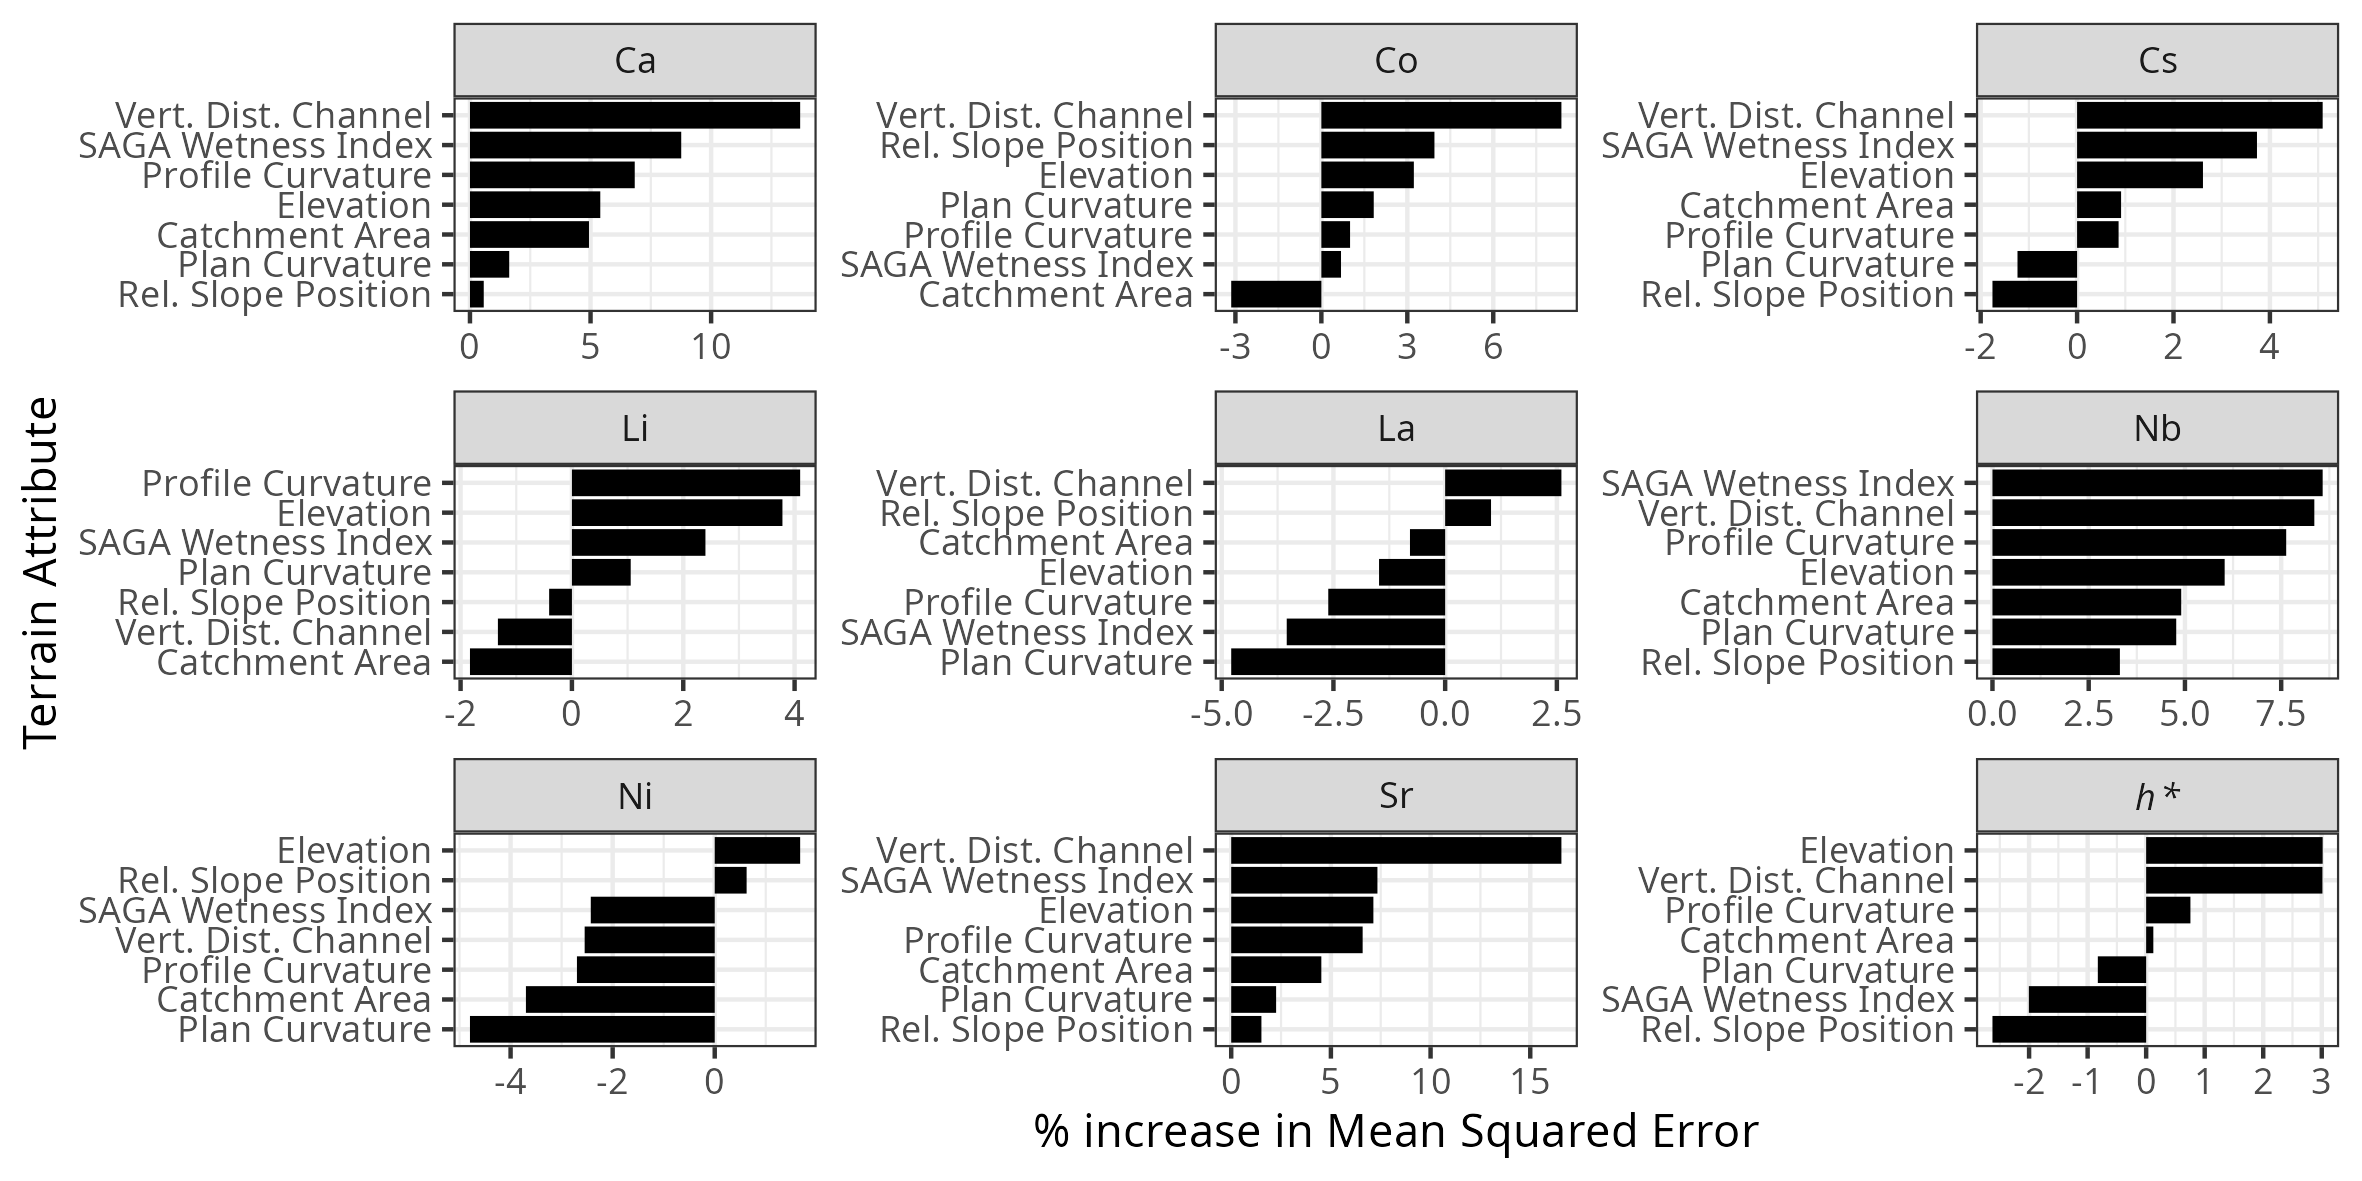
\includegraphics[width=1\linewidth,height=\textheight,keepaspectratio]{images/Forest_RF_summary.png}

}

\caption{\label{suppfig-ag_RF_summary}Variable importance, expressed as
the percentage increase in Mean Squared Error, for soil colour and
geochemical fingerprint properties derived from random forest models
using terrain attributes as predictorsat the forest site.}

\end{suppfig}%

\subsection*{Supplemental tables}\label{supplemental-tables}
\addcontentsline{toc}{subsection}{Supplemental tables}

\begin{supptab}

\caption{\label{supptab-abbrev}Description of spectral reflectance
colour coefficients used as fingerprints. Reproduced from Boudreault et
al.~(2018)}

\centering{

\begin{longtable*}[]{@{}
  >{\raggedright\arraybackslash}p{(\linewidth - 4\tabcolsep) * \real{0.2660}}
  >{\raggedright\arraybackslash}p{(\linewidth - 4\tabcolsep) * \real{0.5532}}
  >{\raggedright\arraybackslash}p{(\linewidth - 4\tabcolsep) * \real{0.1702}}@{}}
\toprule\noalign{}
\begin{minipage}[b]{\linewidth}\raggedright
\textbf{Colour space model}
\end{minipage} & \begin{minipage}[b]{\linewidth}\raggedright
Parameter
\end{minipage} & \begin{minipage}[b]{\linewidth}\raggedright
Abbreviation
\end{minipage} \\
\midrule\noalign{}
\endhead
\bottomrule\noalign{}
\endlastfoot
RGB & Red & R \\
RGB & Green & G \\
RGB & Blue & B \\
CIE xyY & Chromatic Coordinate x & x \\
CIE xyY & Chromatic Coordinate y & y \\
CIE xyY & Brightness & Y \\
CIE XYZ & Virtual component X & X \\
CIE XYZ & Virtual component Z & Z \\
CIE LAB & Metric lightness function & L \\
CIE LAB & Chromatic coordinate opponent red--green scales & \emph{a*} \\
CIE LAB & Chromatic coordinate opponent red--green scales & \emph{b*} \\
CIE LUV & Chromatic coordinate opponent blue--yellow scales &
\emph{u*} \\
CIE LUV & Chromatic oordinate opponent red--green scales & \emph{v*} \\
CIE LCH & CIE hue & \emph{c*} \\
CIE LCH & CIE chroma & \emph{h*} \\
\end{longtable*}

}

\end{supptab}%

\begin{supptab}

\caption{\label{supptab-terrain}Terrain attribute descriptions}

\centering{

\begin{longtable*}[]{@{}
  >{\raggedright\arraybackslash}p{(\linewidth - 2\tabcolsep) * \real{0.0805}}
  >{\raggedright\arraybackslash}p{(\linewidth - 2\tabcolsep) * \real{0.9195}}@{}}
\toprule\noalign{}
\begin{minipage}[b]{\linewidth}\raggedright
Terrain Attribute
\end{minipage} & \begin{minipage}[b]{\linewidth}\raggedright
Description
\end{minipage} \\
\midrule\noalign{}
\endhead
\bottomrule\noalign{}
\endlastfoot
Elevation & Meters above sea level \\
Plan Curvature & Across slope curvature \\
Profile Curvature & Down slope curvature \\
SAGA Wetness Index & Similar to the `Topographic Wetness Index' (TWI),
but it is based on a modified catchment area calculation, which does not
think of the flow as very thin film. As result it predicts for cells
situated in valley floors with a small vertical distance to a channel a
more realistic, higher potential soil moisture compared to the standard
TWI calculation \\
Catchment Area & Area of upslope contributing area \\
Relative Slope Position & A value between 0 and 1 illustrating the
position of a pixel within the landscape with values approaching 0
indicating streams to pits, and values approaching 1 indicating upper
slope positions to peaks \\
Vertical Distance to Channel &
\begin{minipage}[t]{\linewidth}\raggedright
The vertical distance to a channel network base level. The algorithm
consists of two major steps:

1. Interpolation of a channel network base level elevation\\
2. Subtraction of this base level from the original elevations\strut
\end{minipage} \\
\end{longtable*}

}

\end{supptab}%





\end{document}
